\section{Une étude de cas : Cholesky}\label{chap:contribs:apps:cholesky}

Afin de mettre en application nos analyses nous avons choisi comme cas d'étude une application d'algèbre linéaire populaire et bien connue : la factorisation de Cholesky.

On va étudier en détail son exécution et ses parties critiques, et comment on a pu améliorer son exécution, donc il faut expliquer l'algo

\subsection{Description générale}

Factorisation d'une matrice symétrique définie positive, par bloc.


On peut caractériser une factorisation par sa taille de bloc et sa largeur en nombre de blocs.

cf diagram, repose sur quatres noyaux, décrit ci après

\begin{figure}[ht]
  \centering
  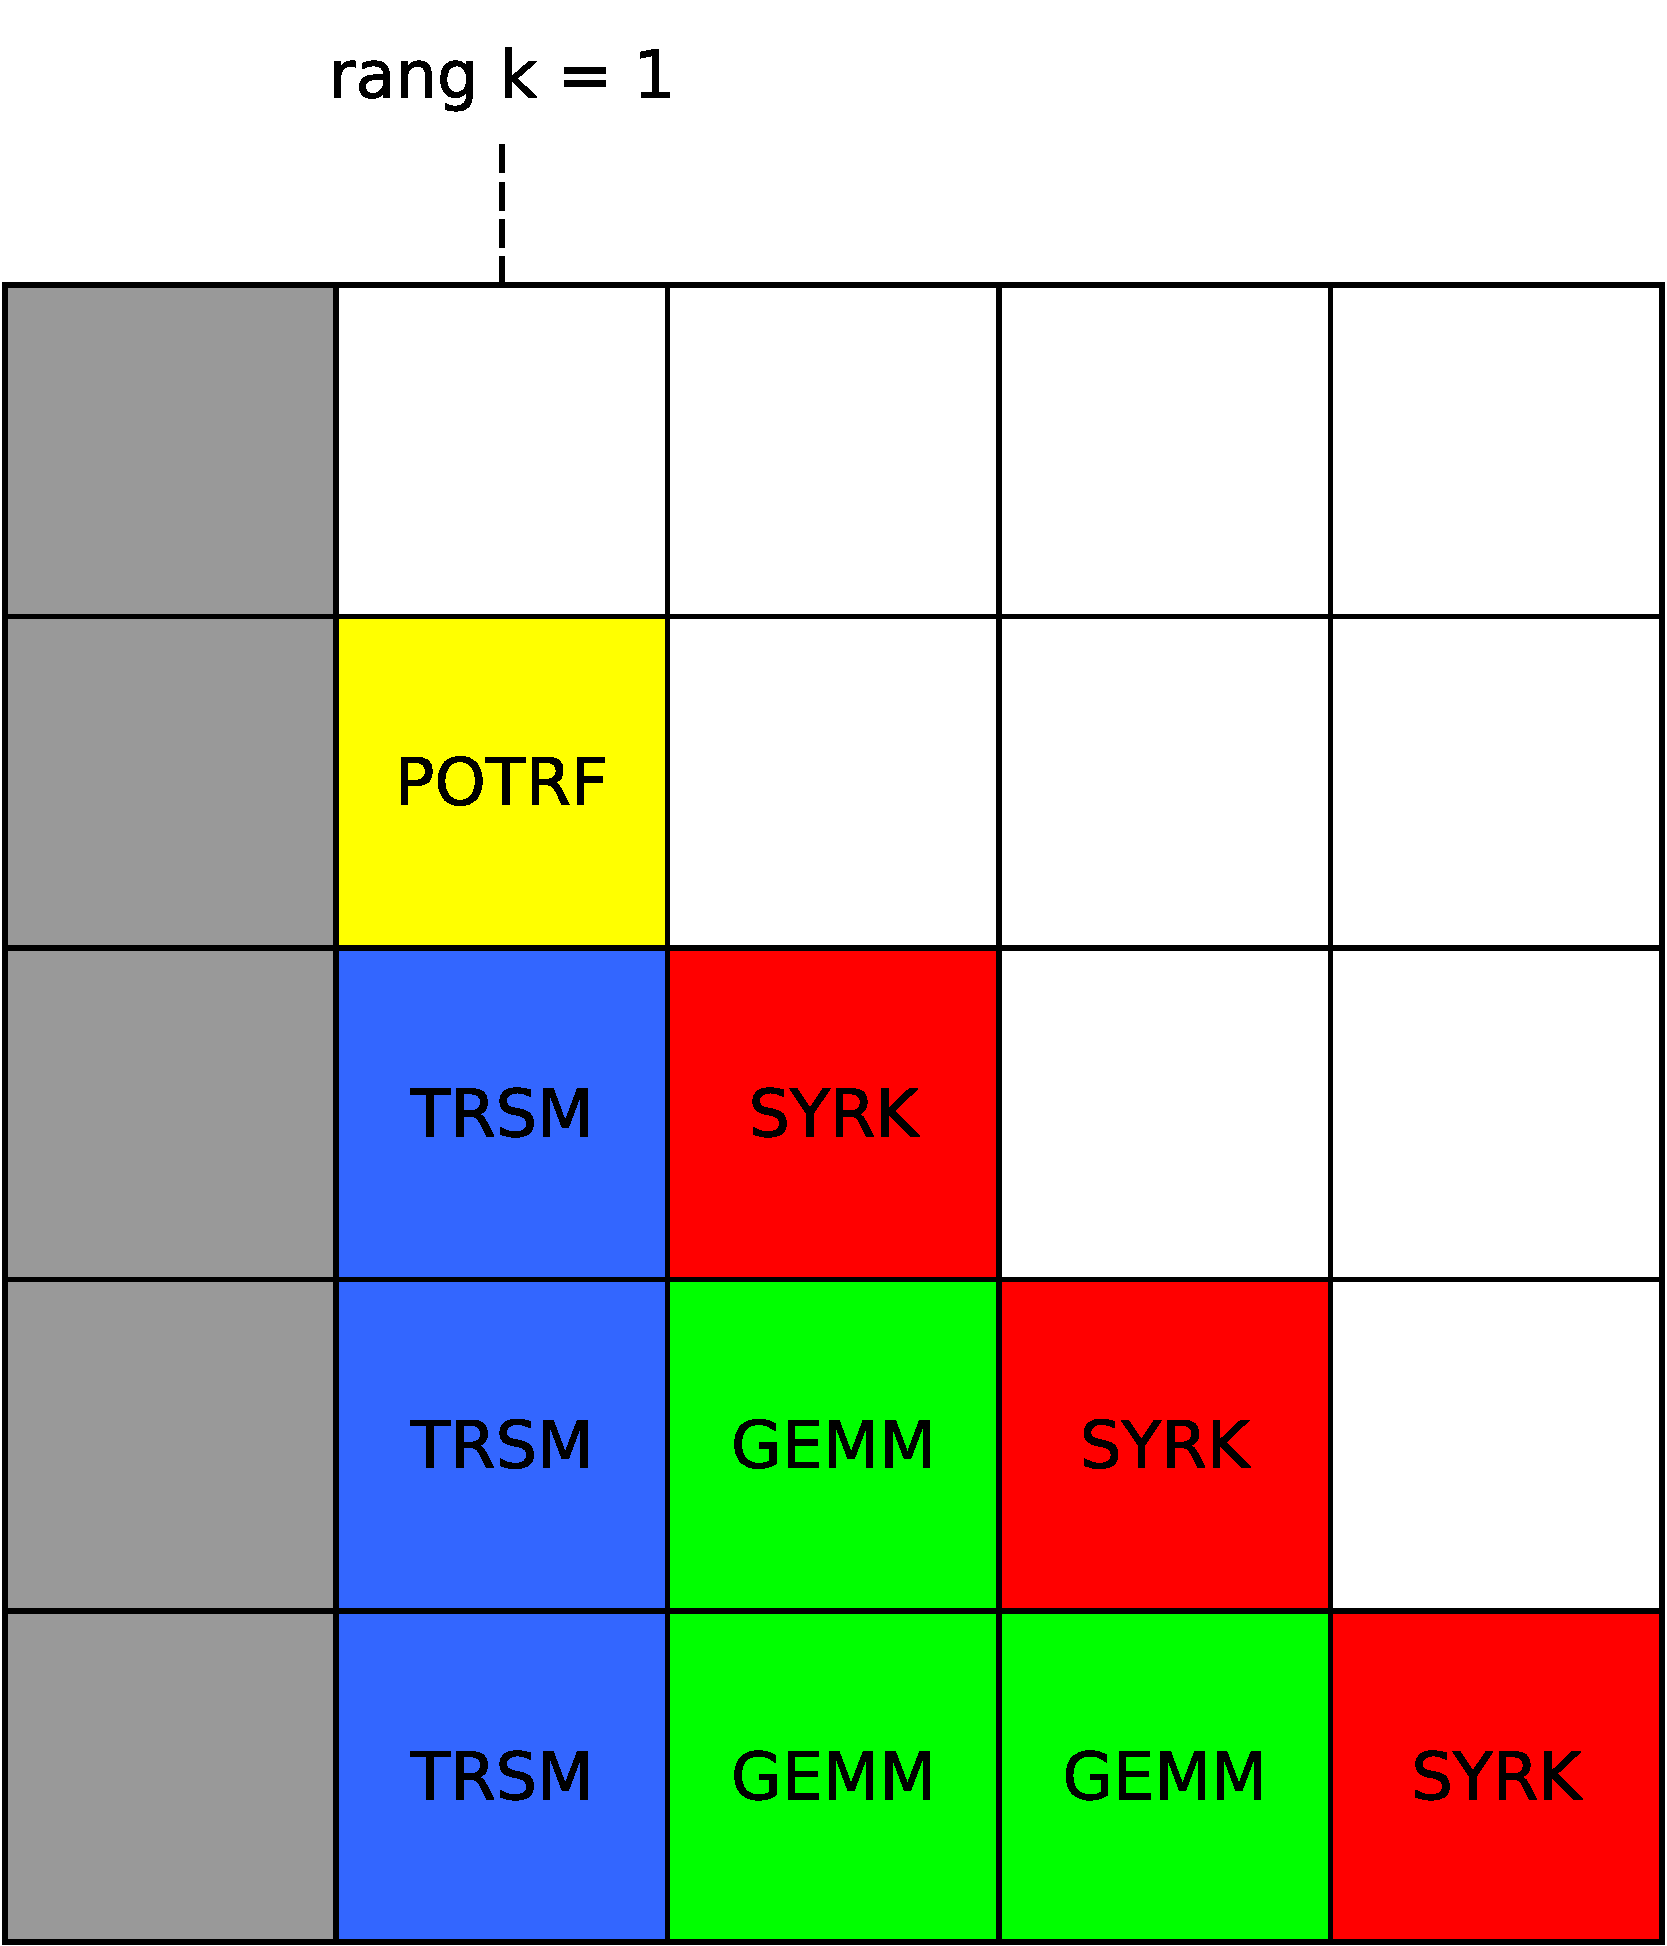
\includegraphics[width=0.6\textwidth]{cholesky-rank-update}
  \caption{Itération du rang k de la factorisation de Cholesky}\label{fig:contribs:apps:cholesky:rank-update}
\end{figure}

À chaque itération on fait les trucs décrit sur la figure~\ref{fig:contribs:apps:cholesky:rank-update}

\paragraph{potrf}

(ou dpotrf pour des |double|)

Cholesky pur sur un bloc

\paragraph{trsm}

Mise à jour du panneau sous le dpotrf (colonne), triangular solve A X = B

\paragraph{syrk}

Maj des sous matrice diagonale (multiplication de matrice triangulaire)

\paragraph{gemm}

\subsection{Graphe de dépendances}

\begin{todo}
graph de dépendances cholesky 5x5
\end{todo}

Décrire aussi dépendances de chaque tâche


maj des sous matrices diagonales restantes

TODO : décrire en détail l'algorithme de Cholesky, et faire un point sur les différentes performances que l'on obtient en fonction de comment on fait varier l'initialisation de données.

GRAPHE : 4.2.4 schéma du DAG de Cholesky, un joli graph en couleur avec une couleur par noyau. point bonus pour un schéma explicatif du fait que dpotrf est la clé pour générer le parallélisme.

GRAPHE : 4.2.4 performances détaillées Cholesky : impact de la taille de la matrice, de la taille de bloc, de la machine. tailles = 8k, 16k, 32k, bs = 128/256/512. (*sans* affinité, juste un topo)

